\documentclass[10pt]{beamer}

\usetheme{default}

\usepackage[utf8]{inputenc}
\usepackage[russian]{babel}
\usepackage[OT1]{fontenc}
\usepackage{amsmath}
\usepackage{amsfonts}
\usepackage{amssymb}
\usepackage{graphicx}
\usepackage{etoolbox}
\usepackage{caption}
\usepackage{subcaption}
\usepackage{pifont}
\usepackage{xcolor}
\usepackage{framed}
\definecolor{shadecolor}{cmyk}{0,0,0,1}
\usepackage{listings}

\lstset{
    backgroundcolor=\color{lightgray},
    commentstyle=\color{blue},
    frame=single
    breakatwhitespace, 
    language=python, 
    columns=fullflexible, 
    keepspaces, 
    breaklines, 
    tabsize=3, 
    subfigurehowstringspaces=false, 
    extendedchars=true,
    numbers=left
}

\makeatletter

\setbeamercolor{title}{fg=white}
\setbeamercolor{frametitle}{fg=black}
\setbeamerfont*{title}{family=\sffamily,size=\LARGE}

\setbeamerfont{page number in head/foot}{size=\scriptsize}
\setbeamertemplate{footline}[frame number]
\let\otp\titlepage
\renewcommand{\titlepage}{\otp\addtocounter{framenumber}{-1}}

\setbeamertemplate{background canvas}{%
	\ifnumequal{\c@framenumber}{0}{%
      
\includegraphics[width=\paperwidth,height=\paperheight]{images/cover.png}
   }{%
      \ifnumequal{\c@framenumber}{\inserttotalframenumber}{
         
\includegraphics[width=\paperwidth,height=\paperheight]{images/back.png}
      }{%
         % Other frames
      }%
   }%
}

\makeatother

\beamertemplatenavigationsymbolsempty

\author{Владимир Гулин}
\title{\newline \newline \newline Лекция 8 \\ Методы снижения размерности}

\begin{document}

\defverbatim[colored]\forsel{%
\begin{lstlisting}[tabsize=4,basicstyle=\ttfamily]
function forwardselection(F, J, n):
    # F - original feature set
    # J - external criterion
    # n - parameter
    initialize F_0 = {} # empty set
    initialize Q = J(F_0) # compute score
    for j in 1..D:
        fbest = find_best_feature(J, F_j-1, F)
        F_j = add_new_feature(F_j-1, fbest) # add feature 
        if J(F_j) < Q:
            jbest = j
            Q = J(F_j) # save best
        if j - jbest >= n:
            return F_jbest
\end{lstlisting}
}

\begin{frame}[plain]
\titlepage
\end{frame}

\begin{frame}{Владимир Гулин}

\begin{center}
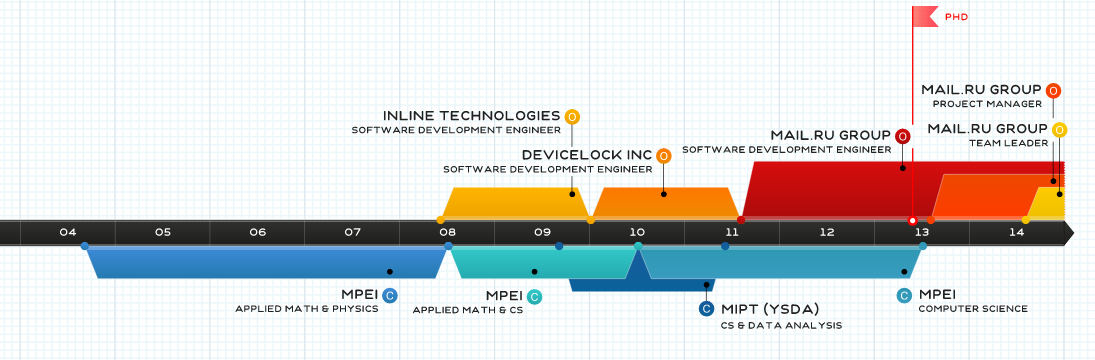
\includegraphics[scale=0.3]{images/timeline_gulin.png}
\end{center}

\begin{footnotesize}
e-mail: \href{mailto:v.gulin@corp.mail.ru}{v.gulin@corp.mail.ru} \\
тел.: +7 (915) 416-95-75
\end{footnotesize}

\end{frame}

\begin{frame}{Структура курса}

{\small
Модуль 1
\begin{enumerate}
\item Задачи Data Mining (Николай Анохин)
\item Задача кластеризации и EM-алгоритм (Николай Анохин)
\item Различные алгоритмы кластеризации (Николай Анохин){\color{red}$^{H}$}
\item Задача классификации (Николай Анохин)
\item Naive Bayes (Николай Анохин)
\item Линейные модели (Николай Анохин)
\item Метод опорных векторов (Николай Анохин){\color{red}$^{HP}$}
\end{enumerate}

Модуль 2
\begin{enumerate}
\item \textbf{Снижение размерности пространства (Владимир Гулин)}
\item \textbf{Алгоритмические композиции 1 (Владимир Гулин)}
\item \textbf{Алгоритмические композиции 2 (Владимир Гулин){\color{red}$^{H}$}i}
\item Нейросети, обучение с учителем (Павел Нестеров){\color{red}$^{H}$}
\item Нейросети, обучение без учителя (Павел Нестеров)
\item Нейросети, глубокие сети (Павел Нестеров)
\end{enumerate}
}

\end{frame}

\begin{frame}{План лекции}
\tableofcontents
\end{frame}

% =======================
\section{Мотивация}
% =======================

\begin{frame}{Мотивация}
\begin{itemize}
\item Визуализация
\item Скорость обучения
\item Качество обучения
\item Экономия при эксплуатации
\item Понимание данных и гибкость построения новых моделей
\end{itemize}
\end{frame}

\begin{frame}{Проклятие размерности (curse of dimensionality)}
\begin{itemize}
\item Сложность вычислений возрастает экспоненциально
\item Требуется хранить огромное количество данных
\item Большое число признаков являются шумными
\item В линейных классификаторах увеличение числа признаков приводит к
    мультиколлинеарности и переобучению.
\item Для метрических классификаторов (в пространсвах с $l_p$ нормой) согласно
    закону больших чисел расстояния становятся неинформативны.
\end{itemize}

\begin{center}
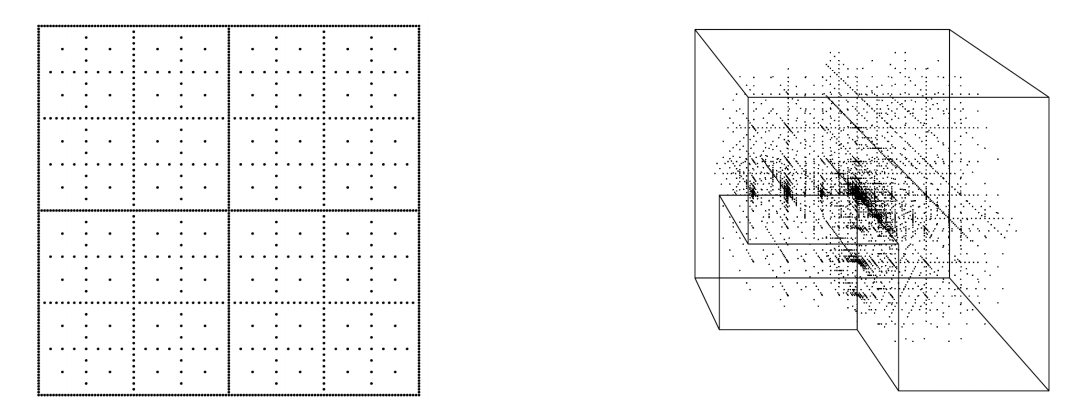
\includegraphics[scale=0.3]{images/cod.png}
\end{center}

\end{frame}

\begin{frame}{Подходы к снижению размерности}

\begin{columns}[C]
        \centering
        \begin{column}{.5\textwidth} 
                \begin{block}{Feature Extraction}
                Data space $\rightarrow$ Feature space\\
                Пространство данных может быть представлено
                сокращенным количеством ``эффективных'' признаков
                \begin{center}
                    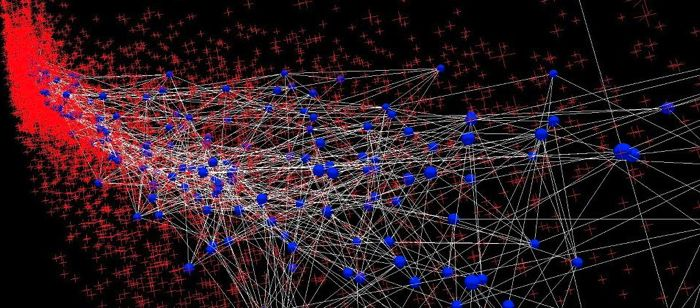
\includegraphics[scale=0.2]{images/gng.jpg}
                \end{center}
                \end{block}
        \end{column}%        
        \begin{column}{.5\textwidth}
                \begin{block}{Feature Selection}
                Data space $\rightarrow$ Data subspace\\
                Отбирается некоторое подмножество наиболее
                ``полезных'' признаков
                \begin{center}
                    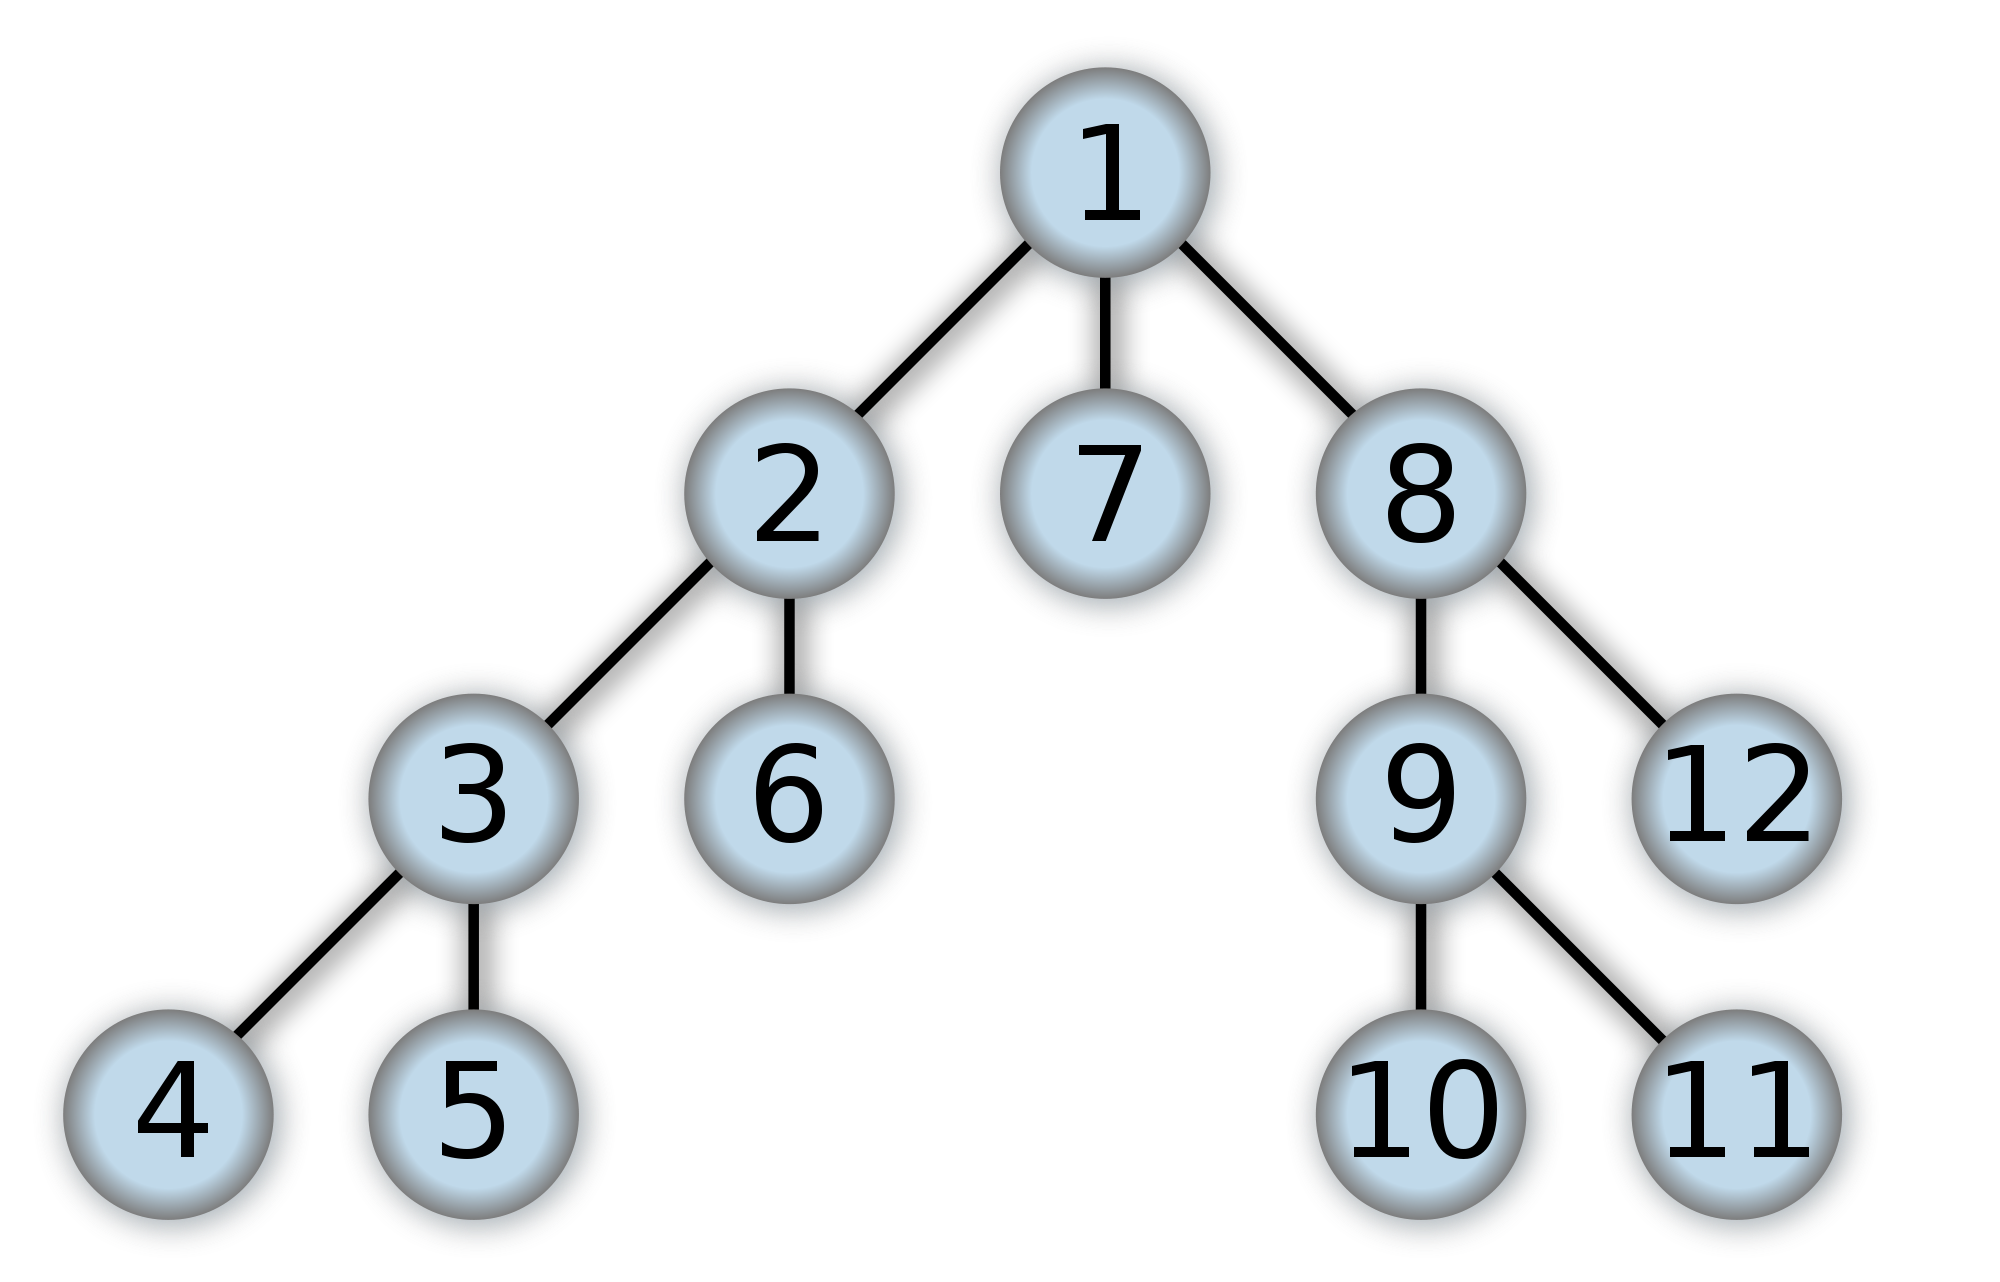
\includegraphics[scale=0.06]{images/dfs.png}
                \end{center}
                \end{block}
        \end{column}
\end{columns}

\end{frame}


% =======================
\section{Методы выделения признаков (feature extraction)}
% =======================

\begin{frame}{Задача выделения/синтеза признаков}

\begin{block}{Feature Extraction}
\end{block}

{\bf Дано.} $N$ обучающих $D$-мерных объектов $\mathbf{x}_i \in \mathcal{X}$,
образующих тренировочный набор данных (training data set) $\mathbf{X}$.

\vspace{1em}
{\bf Найти.} Найти преобразование $A: \mathcal{X} \rightarrow
\mathcal{P}$, $dim(\mathcal{P}) = d < D$, сохранив при этом большую часть
``полезной информации'' об $\mathcal{X}$.

\vspace{1em}
Что мы рассмотрим:
\begin{itemize}
\item PCA
\item ICA
\item Autoencoders with bottleneck
\end{itemize}

\end{frame}

\begin{frame}{Principal Component Analysis}
PCA (Principal Component Analysis) - анализ главных компонент. В теории
информации известен также как преобразование Карунена-Лоева.

\vspace{1em}
\begin{columns}[C]
        \begin{column}{.5\textwidth}
            \begin{block}{Суть метода:}
            Ищем гиперплоскость заданной размерности, такую что ошибка проектирования выборки на данную
            гиперплоскость была бы минимальной.
            \end{block}
        \end{column}
        \begin{column}{.5\textwidth}
        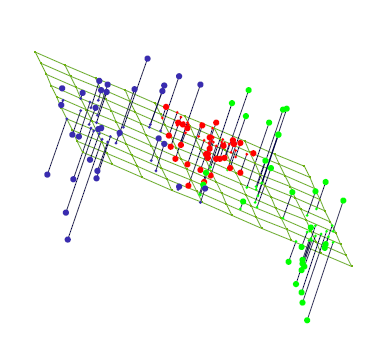
\includegraphics[scale=0.4]{images/projection.png}
        \end{column}
\end{columns}
\end{frame}


\begin{frame}{Principal Component Analysis}
Будем искать преобразование в семействе линейных функций:
\[
    \mathbf{x} = \mathbf{A} \mathbf{p} + \mathbf{b}, \quad \text{где}
\]
\begin{itemize}
    \item $\mathbf{x} \in \mathcal{R}^D$ - представление объекта в исходном
пространстве, 
    \item $\mathbf{p} \in \mathcal{R}^d$ - новые координаты объекта
    \item $\mathbf{b} \in \mathcal{R}^D$, $\mathbf{A} \in \mathcal{R}^{D \times
        d}$
\end{itemize}
\[
    \mathbf{x}_j = \sum \limits _{i=1}^D (\mathbf{x}_j^T \mathbf{a}_i)
    \mathbf{a}_i \quad \text{-  исходные точки}
\]
\[
    \mathbf{\tilde{x}}_j = \sum \limits _{i=1}^d p_{j,i} \mathbf{a}_i + \sum \limits
    _{i=d+1}^D b_i \mathbf{a}_i \quad \text{- проекции}
\]
Тогда критерий выбора гиперплоскости имеет вид:
\[
    J = \frac{1}{N} \sum \limits _{j=1}^N \|\mathbf{x}_j -
    \mathbf{\tilde{x}}_j \|^2 \rightarrow \min \limits _{\mathbf{q},
    \mathbf{z}, \mathbf{b}}
\]
\end{frame}

\begin{frame}{Principal Component Analysis}
\[
    J = \frac{1}{N} \sum \limits _{j=1}^N \|\mathbf{x}_j -
    \mathbf{\tilde{x}}_j \|^2 \rightarrow \min \limits _{\mathbf{q},
    \mathbf{z}, \mathbf{b}}
\]
Несложно показать, что решение будет иметь вид:
\[
    p_{j,i} = \mathbf{x}_j^T \mathbf{a}_i
\]
\[
    b_i = \mathbf{\bar{x}}^T \mathbf{a}_i
\]
где
\[
    \mathbf{\bar{x}} = \frac{1}{N} \sum \limits_{j=1}^{N} \mathbf{x}_j
\]
\[
    \mathbf{R} = cov(\mathbf{X}) = \frac{1}{N} \sum \limits_{j=1}^{N} (\mathbf{x}_j - \mathbf{\bar{x}})^T
    (\mathbf{x}_j - \mathbf{\bar{x}})
\]
$\mathbf{a}_i,\, i=1,\ldots,d$ - базис из собственных векторов ковариационной
матрицы $\mathbf{R}$, отвечающих $d$ наибольших собственным значениям $\lambda_1 \ge
\lambda_2 \ge \ldots \ge \lambda_d$
\end{frame}

\begin{frame}{Иллюстрация PCA}
\begin{figure}
    \centering
    \begin{subfigure}[b]{0.45\textwidth}
        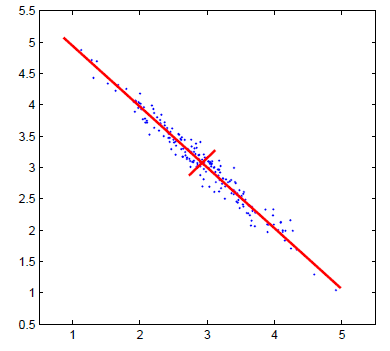
\includegraphics[width=\textwidth]{images/pcasource.png}
    \caption{Исходное пространство}  
    \end{subfigure}
    \begin{subfigure}[b]{0.45\textwidth}
        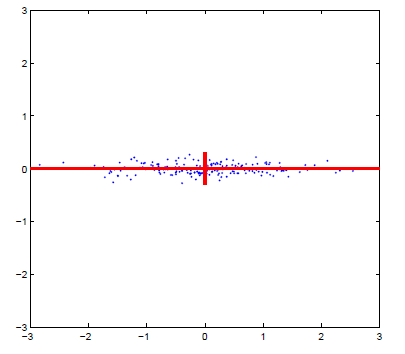
\includegraphics[width=\textwidth]{images/pcaout.png}
    \caption{Итоговое пространство}
    \end{subfigure}
\end{figure}
\begin{itemize}
    \item Сдвигаем начало координат в центр выборки
    \item Поворачиваем оси, чтобы признаки не коррелировали
    \item Избаляемся от координат с малой дисперсией
\end{itemize}
\end{frame}

\begin{frame}{Principal Component Analysis}
    \begin{block}{Альтернативная интерпретация}
        Максимизация дисперсии спроецированных данных
    \end{block}
\begin{center}
    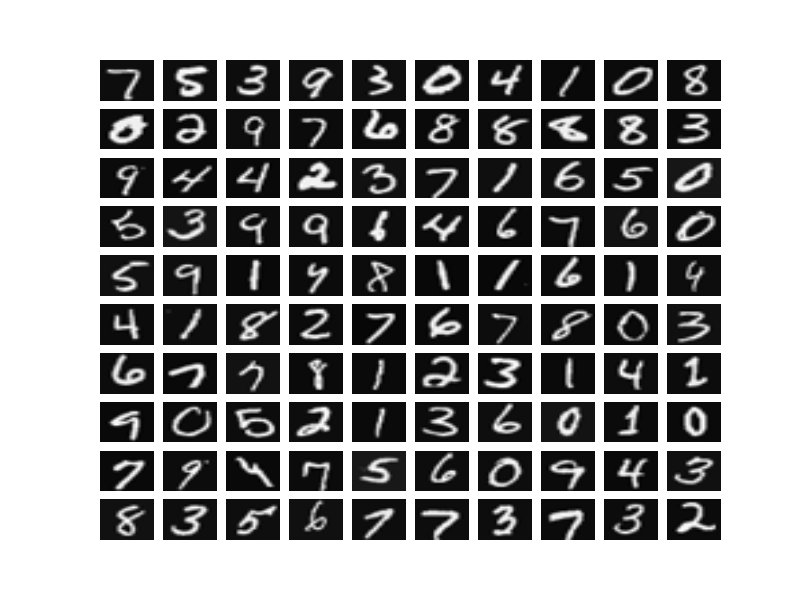
\includegraphics[scale=0.2]{images/digits.png}\\
    Примеры рукописных цифр из базы MNIST
\end{center}

\begin{center}
    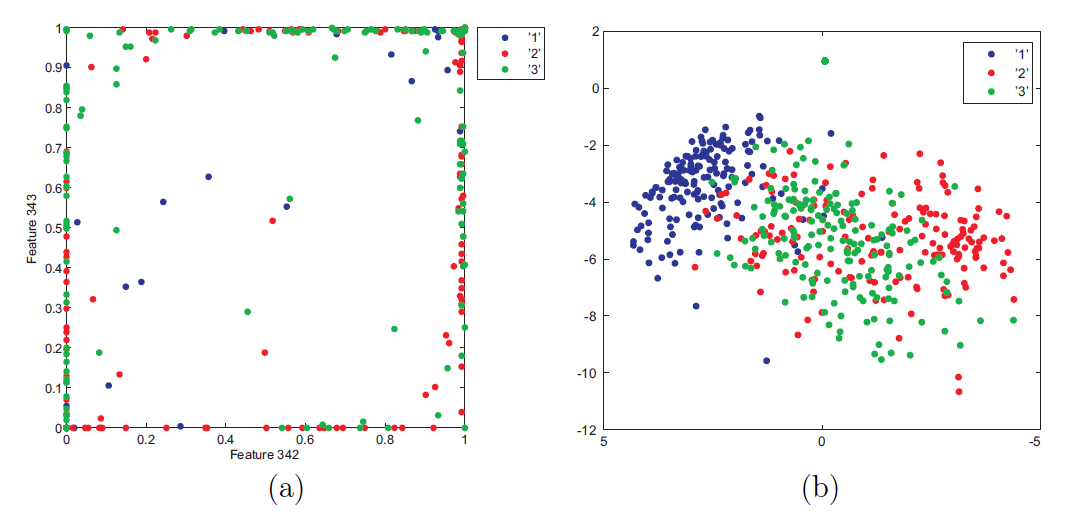
\includegraphics[scale=0.2]{images/pcavsint.png}
\end{center}
\end{frame}

\begin{frame}{Выбор размерности редуцированного пространства}
Поскольку собственные значения ковариационной матрицы $\mathbf{R}$ отсортированы в
порядке убывания $\lambda_1 \ge \lambda_2 \ge \ldots \ge \lambda_d$

\vspace{1em}
\begin{columns}[C]
        \begin{column}{.5\textwidth}
        Критерий выбора размерности будет иметь вид:
        \[
            d: \frac{\sum \limits_{i=1}^{d} \lambda_i}{\sum \limits _{i=1}^{n} \lambda_i} \ge
            \eta, \text{где} \quad \eta=\{0.95, 0.99\}
        \]
        \end{column}
        \begin{column}{.5\textwidth}
            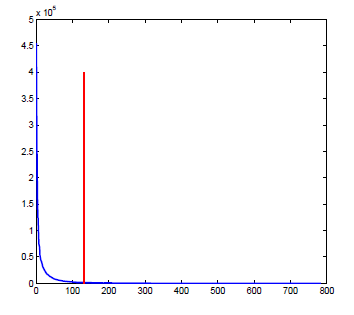
\includegraphics[scale=0.3]{images/numcomp.png}
        \end{column}
\end{columns}
\end{frame}

\begin{frame}{Связь PCA \& SVD}
\[
    \mathbf{X} = \mathbf{U} \mathbf{\Sigma} \mathbf{V}^T
\]
где

$\mathbf{U} (m \times m)$ - ортогональная матрица левых собственных векторов (собственные
вектора матрицы $\mathbf{X} \mathbf{X}^T$ )
    
$\mathbf{V} (n \times n)$ - ортогональная матрица правых собственных векторов (собственные
вектора матрицы $\mathbf{X}^T \mathbf{X}$ )

$\mathbf{\Sigma} (m \times n)$ - диагональная матрица с сингулярными числами на главной диагонали

\vspace{1em}

Матрица главных компонет может быть вычислена:
\[
    \mathbf{X} \mathbf{V} = \mathbf{U} \mathbf{\Sigma} 
\]
\end{frame}

\begin{frame}{Применение PCA}
\begin{figure}
    \centering
    \begin{subfigure}[b]{0.4\textwidth}
        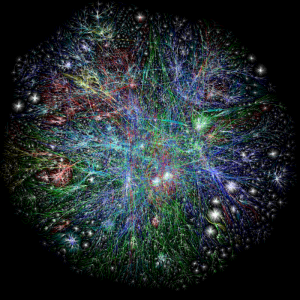
\includegraphics[width=\textwidth]{images/datavisualization.png}
        \caption{Data Visualization}
    \end{subfigure}
    \begin{subfigure}[b]{0.4\textwidth}
        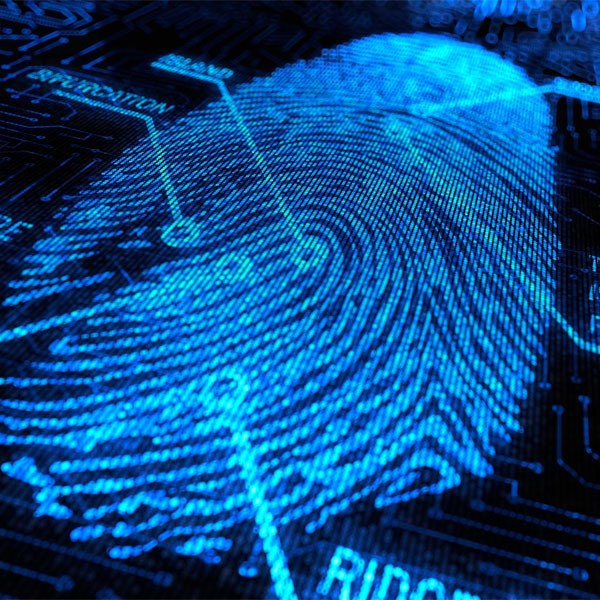
\includegraphics[width=\textwidth]{images/imageprocessing.jpg}
        \caption{Image procesing}
    \end{subfigure}

    \begin{subfigure}[b]{0.4\textwidth}
        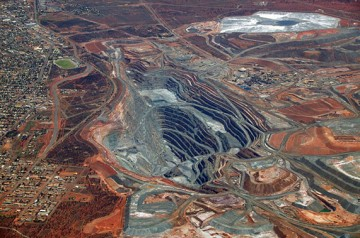
\includegraphics[width=\textwidth]{images/geology.jpg}
        \caption{Prospect}
    \end{subfigure}
    \begin{subfigure}[b]{0.4\textwidth}
        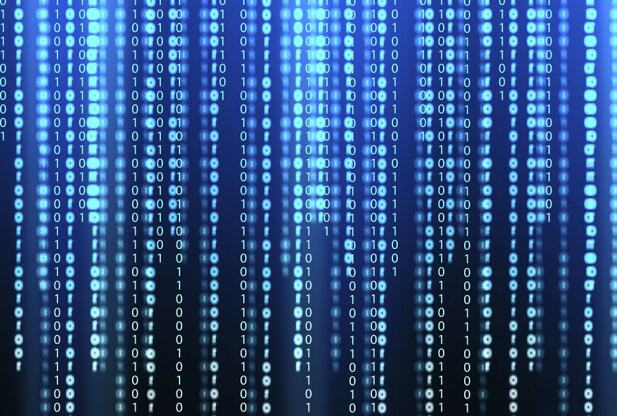
\includegraphics[width=\textwidth]{images/compression.jpg}
        \caption{Data compression}
    \end{subfigure}
\end{figure}
\end{frame}

\begin{frame}{Достоиснтва и недостатки PCA}
\begin{columns}[C]
    \begin{column}{.5\textwidth}
        \begin{itemize}
        \item[+] Алгоритм прост
        \item[+] С помощью ``kernel trick'' адаптируется на нелинейный случай (Kernel
                    PCA)
        \item[---] Проблема с вычислением собсвенных векторов ковариационной матрицы
                    в случае большого количества данных
        \item[---] Координаты объектов в новом пространстве определены неоднозначно
        \end{itemize}
    \end{column}
    \begin{column}{.5\textwidth}
        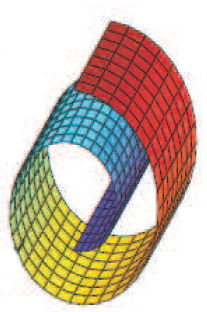
\includegraphics[scale=0.5]{images/surface.png}
    \end{column}
\end{columns}

\begin{block}{Вопрос:}
\begin{itemize}
    \item При каких условиях можно использовать представление данных в виде
        главных компонент для обучения?
\end{itemize}
\end{block}
\end{frame}

\begin{frame}{Задача слепового разделения сигналов}
\begin{center}
    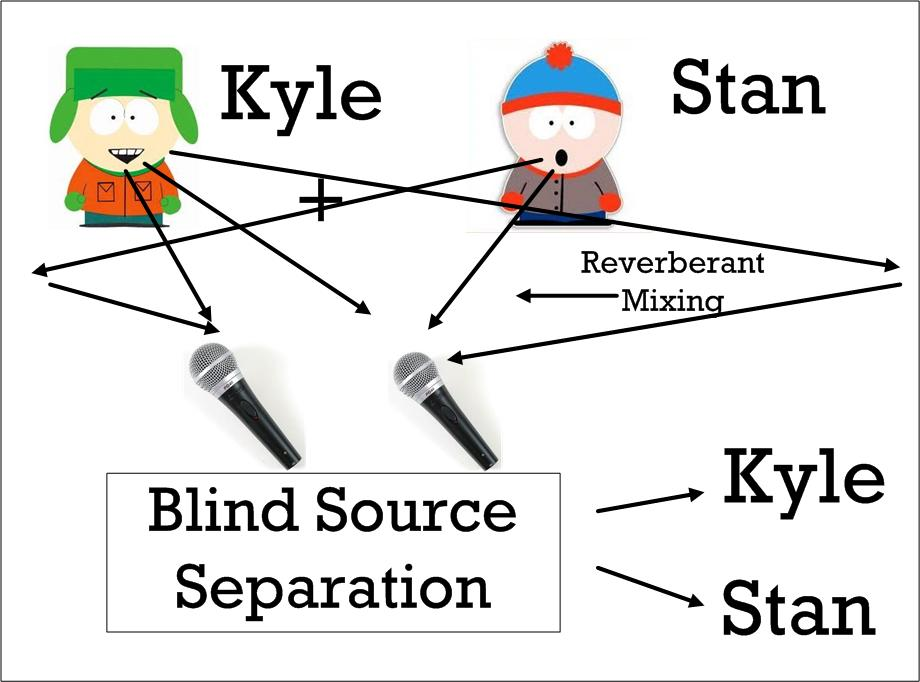
\includegraphics[scale=0.4]{images/sk.jpg}
\end{center}
\end{frame}

\begin{frame}{Independent Component Analysis}
\[
    \mathbf{X}=\mathbf{A} \mathbf{S}
\]
\[
    \mathbf{x}_j = a_{j,1} \mathbf{s}_1 + a_{j,2} \mathbf{s}_2 + \ldots +
    a_{j,N} \mathbf{s}_N, \, j=1,\ldots, N
\]
\begin{itemize}
    \item $\mathbf{x}_j, \mathbf{s}_k$ - случайные величины
    \item $\mathbf{X}$ - наблюдаемые данные
    \item $\mathbf{A}$ - матрица смешивания
    \item $\mathbf{S}$ - неизвестный сигнал
\end{itemize}
\begin{block}{Задача:}
    Оценить $\mathbf{A}$ и восстановить исходные сигналы $\mathbf{S} =
    \mathbf{A}^{-1} \mathbf{X}$.
\end{block}
\begin{block}{Два предположения:}
\begin{itemize}
    \item $\mathbf{s}_i$ статистически независимы $p(\mathbf{s}_1, \mathbf{s}_2) =
        p(\mathbf{s}_1) p(\mathbf{s}_2)$
    \item ``Негауссовость'' распределений
\end{itemize}
\end{block}
\end{frame}

\begin{frame}{Independent Component Analysis}
\begin{block}{Схема}
    \begin{enumerate}
        \item Центрируем данные $\mathbf{x_i} \leftarrow (\mathbf{x_i} -
            \mathbf{\bar{x}}): \mathbf{\bar{x}} \leftarrow \frac{1}{N} \sum
            \limits _{i=1}^N \mathbf{x_i}$
        \item ``Отбеливаем'' данные
        \[
            \mathbf{X} = \mathbf{U} \mathbf{\Sigma} \mathbf{V}^T, \quad \mathbf{X}
            \leftarrow \mathbf{U} \mathbf{\Sigma^{-1/2}} \mathbf{U}^T \mathbf{X}
        \]
        \begin{itemize}
            \item $Cov(\mathbf{X}) = \mathbf{I}$
            \item $\mathbf{A} \mathbf{A}^T = \mathbf{I}$
        \end{itemize}
        \item Находим ортогональную матрицу $\mathbf{A}$
        \begin{itemize}
            \item Infomax
            \item FastICA
            \item JADE
        \end{itemize}
    \end{enumerate}
\end{block}
\end{frame}

\begin{frame}{PCA vs ICA}
    \begin{block}{Геометрическая интерпретация}
        \begin{figure}
            \begin{subfigure}[b]{0.45\textwidth}
            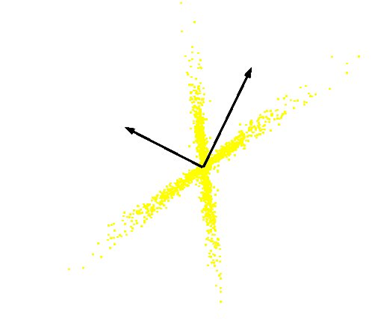
\includegraphics[scale=0.5]{images/pcadirections.png}
            \caption{PCA\\(ортогональны)}
            \end{subfigure}
            \begin{subfigure}[b]{0.45\textwidth}
                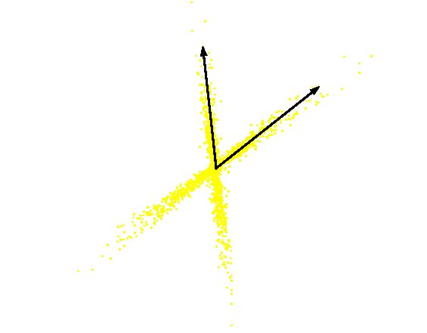
\includegraphics[scale=0.5]{images/icadirections.png}
                \caption{ICA\\(не ортогональны)}
            \end{subfigure}
        \end{figure}
    \end{block}
\end{frame}

\begin{frame}{PCA vs ICA}
\[
    \left[ \begin{array}{c}
            x_1 \\
            x_2
            \end{array}
                \right] = 
    \left[
        \begin{array}{cc}
            a_{11} & a_{12} \\
            a_{21} & a_{22}
        \end{array}
    \right]
    \left[ \begin{array}{c}
            s_1 \\
            s_2
        \end{array}
    \right]
\]
\begin{center}
    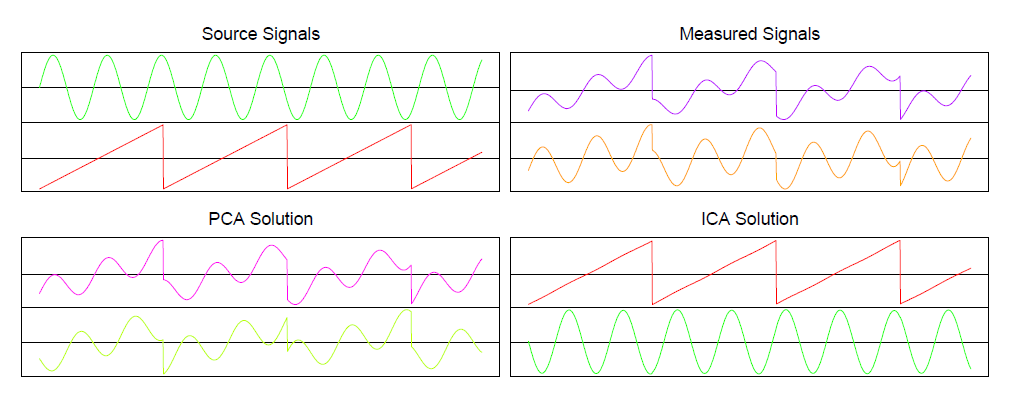
\includegraphics[scale=0.3]{images/pcavsica.png}
\end{center}

\begin{itemize}
    \item Сравнение PCA vs ICA на искуственном временном ряде,
            смоделированном по 1000 равномерно расспределенным точкам.
\end{itemize}
\end{frame}

\begin{frame}{Применение ICA}
\begin{figure}
    \centering
    \begin{subfigure}[b]{0.4\textwidth}
        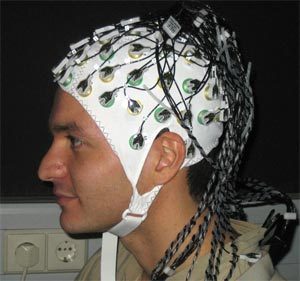
\includegraphics[width=\textwidth]{images/eeg123.jpg}
        \caption{EEG}
    \end{subfigure}
    \begin{subfigure}[b]{0.4\textwidth}
        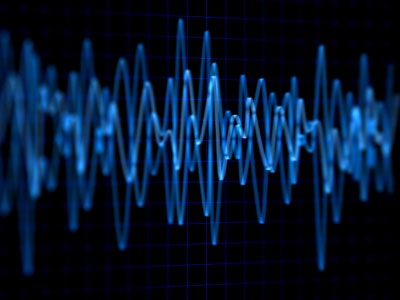
\includegraphics[width=\textwidth]{images/audio.jpg}
        \caption{Audio procesing}
    \end{subfigure}

    \begin{subfigure}[b]{0.4\textwidth}
        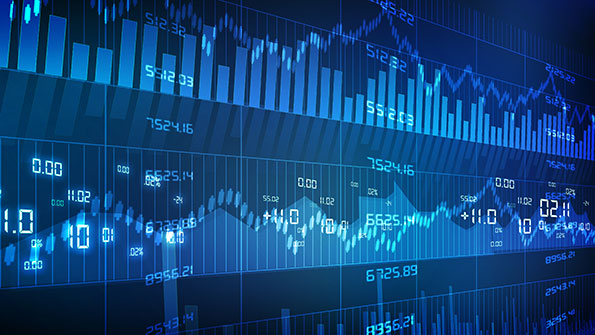
\includegraphics[width=\textwidth]{images/finance.jpg}
        \caption{Finance}
    \end{subfigure}
    \begin{subfigure}[b]{0.4\textwidth}
        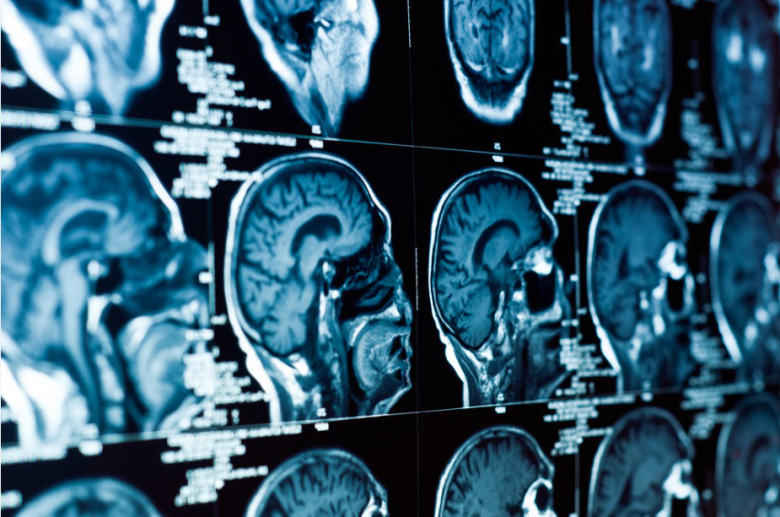
\includegraphics[width=\textwidth]{images/meddata.jpg}
        \caption{Medical data}
    \end{subfigure}
\end{figure}
\end{frame}

\begin{frame}{Методы основанные на автоэнкодерах}
\begin{center}
    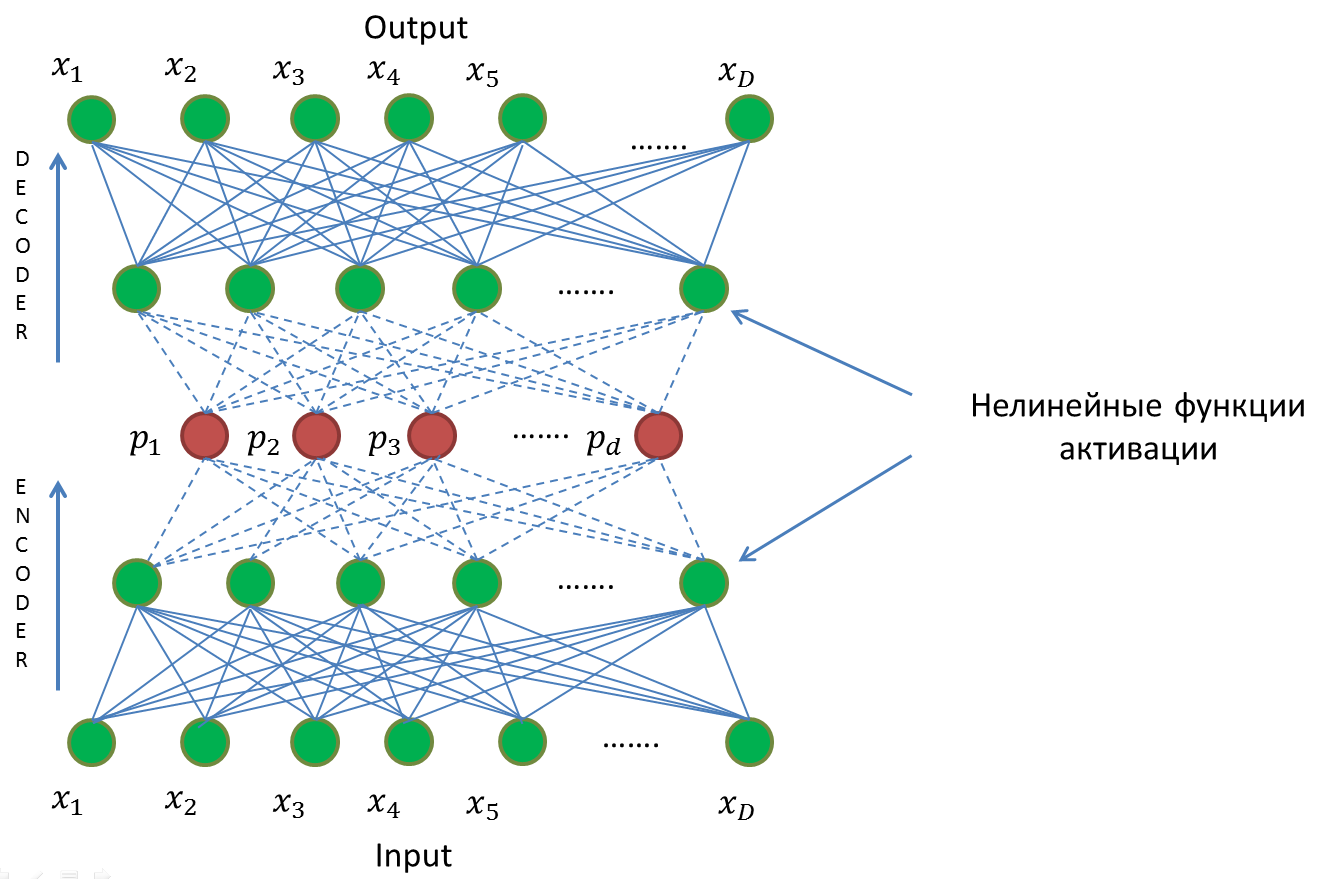
\includegraphics[scale=0.15]{images/autoencoder.png}
\end{center}
\[
    J(\mathbf{w}) = \sum \limits _{i=1}^{N} \| f(\mathbf{x}_i, \mathbf{w}) -
    \mathbf{x}_i \|^2 \rightarrow \min
\]
\begin{block}{Замечание}
Если в сети всего один скрытый слой, тогда результат эквивалентен PCA.
\end{block}
\end{frame}

\begin{frame}{PCA vs Autoencoder}
\begin{block}{Задача визуализации тематических текстовых документов}
\begin{itemize}
\item $D=2000$ - ``мешок слов''
\item $N=4 \cdot 10^5$ документов
\end{itemize}
\end{block}
\begin{figure}
    \centering
    \begin{subfigure}[b]{0.45\textwidth}
        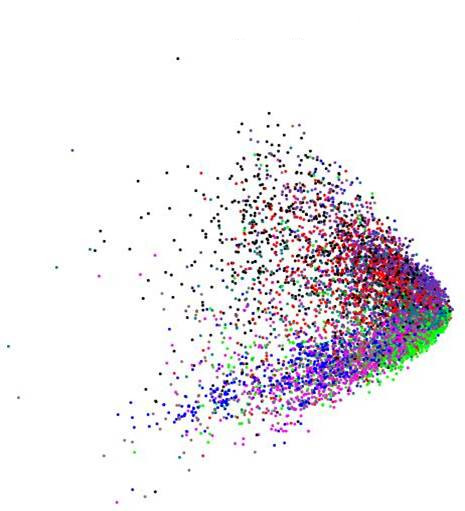
\includegraphics[width=\textwidth]{images/hpca.jpg}
        \caption{PCA}
    \end{subfigure}
    \begin{subfigure}[b]{0.45\textwidth}
        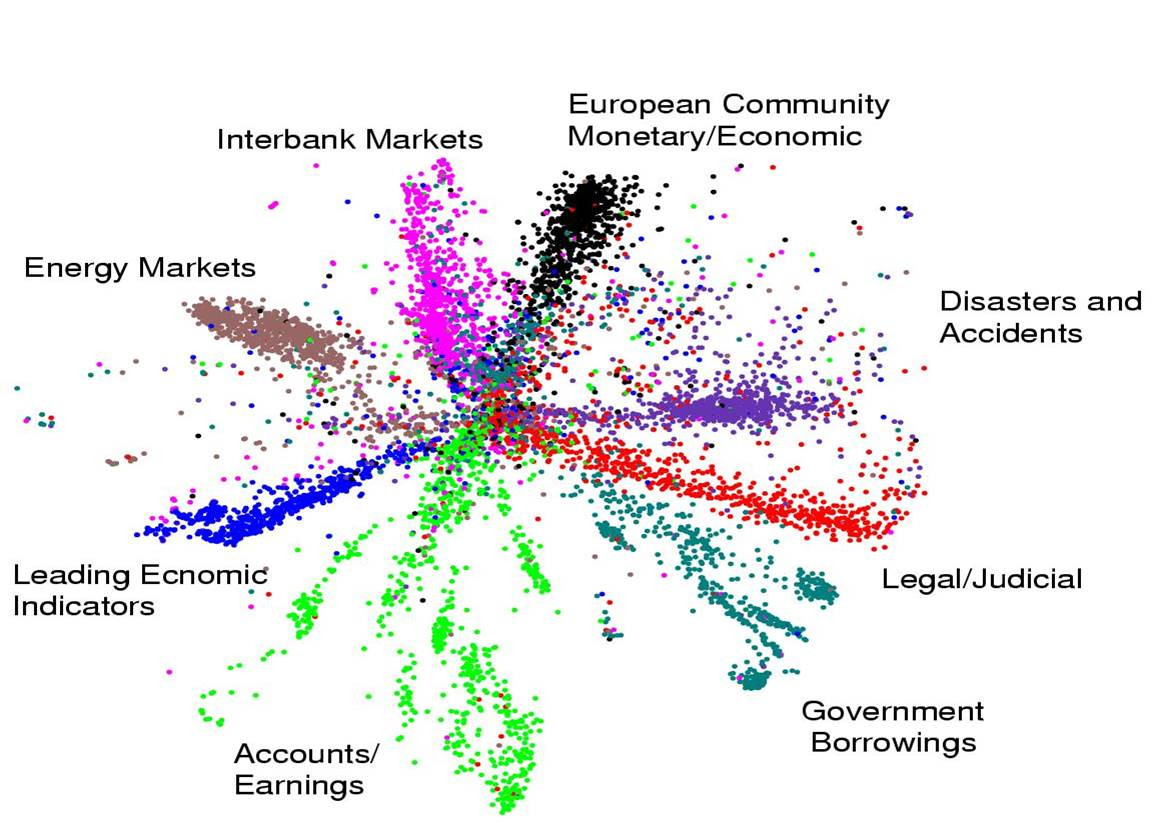
\includegraphics[width=\textwidth]{images/hauto.jpg}
        \caption{Deep Autoencoder}
    \end{subfigure}
\end{figure}
\end{frame}

\begin{frame}{``Бабушкин'' нейрон}
%Сказ про то как Ng c корешами мутил автоэнкодер девятислойный...
\begin{columns}[C]
    \begin{column}{.5\textwidth}
    \begin{itemize}
    \item Andrew Ng
    \item 9-ти слойный разряженный автоэнкодер
    \item Асинхронный градиентный спуск
    \item 10 млн. кадров случайно взятых из роликов youtube
    \item Удалось найти нейрон, отвечающий за наличие лица в кадре
    \end{itemize}
    \end{column}
    \begin{column}{.5\textwidth}
    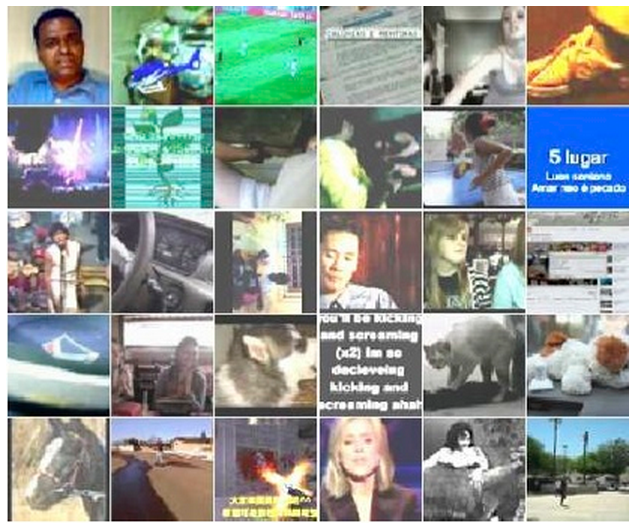
\includegraphics[width=\textwidth]{images/youtube.png}
    \end{column}
\end{columns}
\end{frame}

% =======================
\section{Методы отбора признаков (feature selection)}
% =======================

\begin{frame}{Задача отбора признаков}
\begin{block}{Feature Selection}
\end{block}

{\bf Дано.} $N$ обучающих $D$-мерных объектов $\mathbf{x}_i \in \mathcal{X}$,
образующих тренировочный набор данных (training data set) $\mathbf{X}$, а также каждому
$\mathbf{x}_i$ соответсвует метка $c_i \in \mathcal{R}$.

\vspace{1em}
{\bf Найти.} Найти подмножество признаков $F$ исходного признакового пространства
$\mathcal{F} = \{f_1, f_2, \ldots, f_D \}$, содержащее наиболее ``информативные'' признаки.

\vspace{1em}
Что мы рассмотрим:
\begin{itemize}
    \item Переборные алгоритмы
    \item Методы основанные на корреляции/взаимной информации
    \item Embedded methods
\end{itemize}

\end{frame}

\begin{frame}{Отбор признаков ``в лоб''}
\begin{center}
    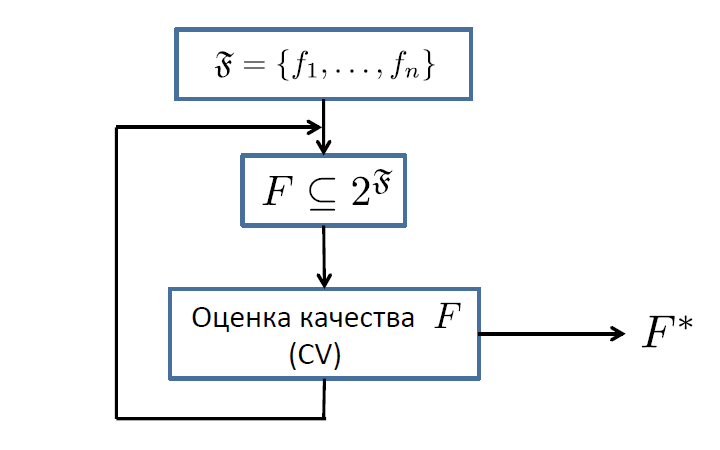
\includegraphics[scale=0.3]{images/featureselection.png}
\end{center}
\begin{itemize}
    \item Экспертный подход
    \item Full Search (NP hard)
    \item Жадные алгоритмы (Forward selection, Backward elimination, Bidirectional
            elimination etc.)
\end{itemize}
\end{frame}

\begin{frame}{Жадные алгоритмы отбора признаков}
    \begin{block}{Forward selection}
    \forsel
    \end{block}
    \begin{block}{Backward elimination}
    \begin{itemize}
        \item Все аналогично. Только ислючаем
    \end{itemize}
    \end{block}
\end{frame}

\begin{frame}{Жадные алгоритмы отбора признаков}
\begin{block}{DFS. Основные идеи:}
\begin{itemize}
    \item Избегаем повторов при переборе
    \item Если подмножество признаков бесперспективно, то не будем пытаться
            его дальше наращивать. 
\end{itemize}
\end{block}
\begin{center}
    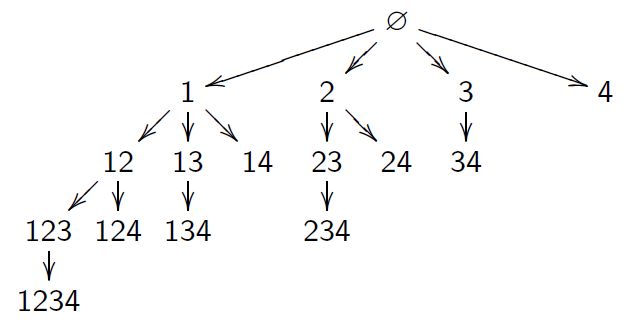
\includegraphics[scale=0.3]{images/searchtree.png}
\end{center}

Оценка бесперспективности:
\[
    \exists j: \quad J(F) \ge \eta J(F_j^*), \quad |F| \ge j+n
\]
\end{frame}

\begin{frame}{Жадные алгоритмы отбора признаков}
    \begin{block}{Итоги}
    \begin{itemize}
        \item Не все признаки ``полезны''
        \item Отбор признаков проводится по внешним критериям (СV)
        \item Для сокращения перебора хороши любые эвристики
        \item Предполагаем, что перебор по подмножествам устойчив
        \item \textcolor{red}{{НАДО ПЕРЕОБУЧАТЬ АЛГОРИТМ}}
    \end{itemize}
    \end{block}
\end{frame}

\begin{frame}{Методы основанные на корреляции/взаимной информации}
Коэффициент корреляции
\[
    r(X,Y) = \frac{\sum \limits _x (x - \bar{x}) \sum \limits _y (y -
    \bar{y})}{\sqrt{ \sum \limits _x (x - \bar{x})^2  } \sqrt{ \sum \limits _y
(y - \bar{y})^2  } }
\]
\begin{itemize}
    \item Correlation feature selection (cfs)
\end{itemize}

\vspace{1em}
Взаимная информация
\[
    I(X,Y) = \sum \limits _x \sum \limits _y p(x,y) \log \left(
    \frac{p(x,y)}{p(x)p(y)} \right)
\]
\begin{itemize}
    \item Minimum redundancy maximum relevance (mRMR)
\end{itemize}
\end{frame}

\begin{frame}{mRMR}
\begin{block}{Идея}
\begin{itemize}
\item Будем отбирать признаки, которые имеют наибольшую взаимную информацию с
    ответами
\item Будем штрафовать признаки за избыточность, в контексте уже отобранных
    фичей
\end{itemize}
\end{block}
\[
    Relevance(F, c) = \frac{1}{|F|} \sum \limits _{f_i \in F} I(f_i, c) 
\]
\[
    Redundancy(F) = \frac{1}{|F|^2} \sum \limits _{f_i, f_j \in F} I(f_i, f_j)
\]
Тогда критерий mRMR имеет вид:
\[
    mRMR = \max \limits _F (Relevance(F, c) - Redundancy(F))
\]
\end{frame}

\begin{frame}{Embedded methods}
Что мы уже знаем?
\begin{itemize}
    \item Sparse regression, LASSO
    \item Decision Trees with pruning
    \item Autoencoders with bottleneck
\end{itemize}

\vspace{1em}
С чем нам еще предстоит познакомиться?
\begin{itemize}
    \item Regularized Random Forest (RRT)
    \item Regularized gradient boosting
    \item Regularized neural nets
\end{itemize}
\end{frame}

\begin{frame}{О чем еще не поговорили?}
\begin{block}{Отбор признаков без учителя}
\end{block}
\begin{block}{Оценка качества фичей}
\end{block}
\end{frame}

\begin{frame}[fragile]{Задача}

{\bf Дано:} Имеется набор трехмерных данных \\
{\bf Требуется:} Построить проэкцию этих данных на плоскость использую любую
пару признаков. Вычислить pca и отобразить данные в пространстве первых двух
собственных векторов.

\vspace{1em}
Пошаговая инструкция
\begin{enumerate}
\item Скачать и запустить шаблон кода на python \url{http://goo.gl/5kW1Pa}
\begin{shaded}
{\color{green} \begin{verbatim}
$ python pca.py -h
$ python pca.py -i 50
\end{verbatim}}
\end{shaded}
\item Заполнить функцию \textsf{compute\_pca}
\item Сгенирировать многомерные данные ($D > 10$). Реализовать критерий выбора
    размерности редуцированного пространства.
\end{enumerate}

\end{frame}

\begin{frame}[plain]
\begin{center}
{\Large Вопросы}
\end{center}
\end{frame}

\end{document}
